\documentclass{standalone}
%<--------------------------------------------------------------------------->%
%%% TikZ %%%
\usepackage{tikz}
% \usetikzlibrary{calc}
% \usetikzlibrary{angles,quotes}
% \usetikzlibrary{intersections,topaths}
% \usetikzlibrary{decorations.markings}
%<--------------------------------------------------------------------------->%

\begin{document}

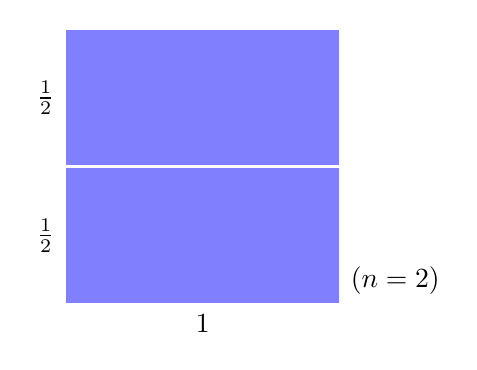
\begin{tikzpicture}[scale=3.5,thick,line cap=round]
	\tikzstyle{jiao}=[solid,circle,draw,fill=white,inner sep=.8pt];
	\tikzstyle{tile1}=[line width=0.1em,draw=white,fill=blue!50];
\tikzstyle{tile2}=[line width=0.1em,draw=white,fill=red!50];
\tikzstyle{tile3}=[line width=0.1em,draw=white,fill=blue!50!red!60];
\tikzstyle{tile4}=[line width=0.1em,draw=white,fill=blue!20!red!60];

	\draw[tile1] (0,0)   rectangle +(1,1/2);
	\draw[tile1] (0,1/2) rectangle +(1,1/2);
	\node[left] at (0,1/4) {$\frac12$};
	\node[left] at (0,3/4) {$\frac12$};
	\node[below] at (1/2,0) {$1$};
	\node[above right] at (1,0) {$(n=2)$};
\end{tikzpicture}

\end{document}
